\part{Preliminary notions}


\section{Physical setup}

    \subsubsection*{Brane-world paradigm}

        We consider our world to be a slice in the ten-dimensional spacetime of type II superstring theory, i.e. the worldvolume of a D$3$-brane. More precisely, we consider a stack of $N$ D$3$-branes in order to have $\U(N)$ Chan-Paton factors resulting in a $\U(N)$ gauge group. To have D$3$-branes, we need to consider type IIB superstring theory. The spacetime is therefore not necessarily $\R^{1,9}$ but of the more general form
        \begin{equation*}
            M = \R^{1,3}\times M^{(6)}.\label{spacetimedecomp}
        \end{equation*}
        This is the so-called \emph{brane-world paradigm}. %In particular, we will be interested in type IIB string theory because of its self-duality under S-duality. \todo{Why ?}

    \subsubsection*{Supersymmetry and Calabi-Yau manifolds}
    
        Independently from string theory, we can ask for the wolrdvolume theory to be supersymmetric. We start from type IIB superstring theory which is $10$-dimensional and has $\mN=2$ supersymmetry so it possesses $32$ supercharges. As usual, they transform under the minimal spinor representation (MSR) of the bulk Lorentz group, here $\SO(1,9)$. In ten dimensions this representation is $8$-dimensional (complex) which is why there are $2(8+8)=32$ supercharges: $8$ transforming in the $8$-dimensional MSR and $8$ transforming in the $8$-dimensional conjugate MSR and whole thing times two since $\mN=2$. If we compactify type II string theory on $\R^{1,3}\times M^{(6)}$ where $M^{(6)}$ is any $6$-dimensional manifold, supersymmetry is broken. The reason for this is that the supercharges now have to transform under the MSR of $\SO(1,3)\times\H(M^{(6)})$\todo{Why ?}, where $\H(M^{(6)})$ is the holonomy group of $M^{6}$. Recall that a generic curved 6-dimensional manifold has $\O(6)$ holonomy and $\SO(6)$ if it is orientable. We only consider the later case. The supercharges must therefore transform under the MSR of $\SO(1,3)\times\SO(6)$. The MSR of $\SO(1,3)$ being $\boldsymbol{2}$ and the one of $\SO(6)$ being $\boldsymbol{4}$, we conclude that imposing the spacetime to have the form \eqref{spacetimedecomp} changes the representation under which the supercharges transform as follows:
        \begin{equation}
            \boldsymbol{8}\oplus\bar{\boldsymbol{8}}\to (\boldsymbol{2}_L,\boldsymbol{4})\oplus(\boldsymbol{2}_R,\bar{\boldsymbol{4}}).
        \end{equation}
        If we stop here, the residual supercharges might be ill-defined since making a tour around a loop in $M^{(6)}$ could result in anon-trivial rotation. To solve this problem, we need also to be more restrictive on the holonomy. In fact, it is precisely the holonomy of the transverse space that dictates the number of supersymmetries that are left. Let us now consider a four-dimensional field theory resulting from compactification of the transverse six-dimensional space. The number of supercharges that generate supersymmetries for this theory is the number of Killing spinor (covariantly constant spinor): each Killing spinor contracted with the local supersymmetry current generates a residual supersymmetry. \todo{Explain.} Now the link with holonomy: since $\SO(6)\cong\SU(4)$, minimal spinors can be viewed as having four complex component and as transforming under $\SU(4)$. Indeed, minimal spinors in six dimensions have four complex components. In order to have one covariantly conserved spinor, we look for the biggest subgroup of $\SU(4)$ that leaves a component of the spinor invariant. This is clearly $\{e\}\times\SU(3)\subset\SU(4)$ that acts trivially on the first component. The spinor $(1,0,0,0)$ is then covariantly conserved. Our transverse space must therefore have $\SU(3)$ holonomy such that the parallel transport of the spinor $(1,0,0,0)$ under any closed loop is a lower $\SU(3)$ rotation. We conclude that if the transverse Calabi-Yau has $\SU(3)$ holonomy, the worldvolume theory has $\mN=1$ supersymmetry. The same reasoning can be used to obtain that $\SU(2)$ holonomy implies $\mN=2$ supersymmetry.

        To conclude, preserving any degree of supersymmetry constrains the transverse space $M^{(6)}$ to be compact, complex, Kähler and to have $G\subset\SU(3)$ holonomy. Namely, $M^{(6)}$ must be a Calabi-Yau threefoldau manifolds are given in appendix \ref{sec:CY}.

    \subsubsection*{Non-compact transverse space}
    
        If we let the worldvolume of the D$3$-branes carry the requisite gauge theory while the bulk contains gravity, we can relax the compactness condition and study non-compact Calabi-Yau threefolds. Using a non-compact transverse space can intuitively be understood as a Kaluza-Klein compactification where we take the size of the compact dimensions to infinity. The four-dimensional gravity coupling constant being inversely proportional to this quantity, there is no gravity in this limit. This makes the analysis much simpler and therefore also serves as an argument to ignore gravity in the worldvolume theory. Consequently, we will mostly ignore gravity and not care about the metric of the spacetime, see appendix \ref{app:spacetimegeom} for more details. In this setup we cannot really talk about compactification anymore. Instead we just think of it as a flat space on which lives the gauge theory while gravity only lives in transverse space. This non-compact limit Kaluza-Klein argument is useful to understand why there no gravity from the point of view of the worldvolume theory.

    \subsubsection*{Singular transverse space}

        The only smooth Calabi-Yau threefold is $\C^3$ so we are lead to consider singular Calabi-Yau varieties. A Calabi-Yau variety is an affine variety that locally models a Calabi-Yau manifold, therefore allowing for singularities. We usually denote $S\equiv M^{(6)}$ to remind us of the singular aspect. String theory being a theory of extended objects, it is well-defined on such singularities. In a sense that will be clarified later, this singular structure of the geometry requires to ``project'' the theory. As a result, the gauge group $\U(N)$ will be broken down into products of smaller gauge groups. The simplest examples of singular Calabi-Yau varieties are Calabi-Yau orbifolds. We will mainly be interested these examples.
    
        From the point of view of the orbifold, the D$3$-brane is a point. Consequently, the D$3$-branes parametrize the transverse space. This is the first clue of the crucial relationship between the worldvolume theory and the Calabi-Yau singularity. Eventually, we will see that the classical vacuum of the gauge theory should be, in explicit coordinates, the defining equation of $S$. This is precisely the opposite of the projection manipulation we mentioned above: recovering the transverse space from the gauge theory. 
        
        Projecting and computing the classical vacua are therefore inverse operations with respect to each other. This suggest a bijection between the singular transverse space and the gauge theory: the former can be computed from the latter and vice-versa. This is called ``forward algorithm'' and ``inverse algorithm''. We will of course discuss this in more details.

    \subsubsection*{Mathematical formulation}

        Mathematically, this brane-world paradigm is the realization of branes as supports of vector bundles (sheaf). Gauge theories on branes are intimately related to algebraic constructions of stable bundles, i.e. holomorphic or algebraic vector bundles that are stable in the sense of geometric invariant theory. In particular, D-brane gauge theories manifest as a natural description of symplectic quotients and their resolutions in geometric invariant theory.

        To summarize in more mathematical terms, our D-branes, together with the stable vector bundle (sheaf) supported thereupon, resolves the transverse Calabi-Yau orbifold which is the vacuum for the gauge theory on the worldvolume as a GIT quotient. \todo{Explain.}

    \subsubsection*{Summary}

        We consider $N$ D$3$-branes in type IIB superstring theory carrying a $\U(N)$ gauge group. The transverse space $S$ is taken to be a non-compact singular Calabi-Yau variety.

    

\section{Supersymmetric Yang-Mills theories}

    \subsection{Vacua space of SYM}

        Let us consider a supersymmetric gauge theory in $d=4$ with $k$ chiral sueprfields $\Phi_i$ ($i=1,\dots,k$) charged under the gauge group $G$ in an arbitrary representation $r_i$, in which the generators of $G$ are given by $T^a_{r_i}$ ($a=1,\dots,\dim G$). $\mathcal{W}_\alpha$ is the gaugina chiral superfield, containing the field strength. The lagrangian density on superspace is given by
        \begin{equation}
            \mathcal{L}=\int\d^2\theta\d^2\bar{\theta}~\Phi^\dagger e^{2V}\Phi+\int\d^2\theta\left\{\frac{\tau}{16\pi i}\tr(\mathcal{W}^\alpha\mathcal{W}_\alpha)+W(\Phi)\right\}+\text{c.c.}
        \end{equation}
        where we ignored the gauge indices. The superpotential $W(\Phi)$ is a holomorphic polynomial in the $\Phi_i$. The space of vacua is the space of configurations of $\Phi$ such that the $D$-terms and the $F$-terms vanish:
        \begin{subequations}
            \begin{empheq}[box=\widefbox]{align}
                D^a &\equiv \sum_i\Phi^\dagger_iT^a_{r_i}\Phi^i = 0,\\
                F^\dagger_i&\equiv \pdv{W}{\Phi^i}=0.
            \end{empheq}
        \end{subequations}
        In turns out that the full space of vacua of any supersymmetric gauge theory can be described as an algebraic variety.
    
    \subsection{$\mN=4$ super Yang-Mills theory in $D=4$}\label{sec:N4SCFT}

        \subsubsection{Superconformal group $\SU(2,2|4)$ and its representations}

            Conformal transformations and supersymmetries do not commute so the presence of conformal symmetry in addition to $\mN=4$ supersymmetry leads to an even larger group of symmetry known as the \emph{superconformal group}. In the $D=4,\mN=4$ case, the superconformal group is the super group\footnote{Supermanifold which is also a group with smooth product and inverse maps.} $\SU(2,2|4)$. The different component of the latter are
            \begin{itemize}
                \item \textbf{Conformal symmetries}: they form the 15-dimensional subgroup $\SO(2,4)$ and are generated by $P_\mu,M_{\mu\nu},K_\mu$ and $D$.
                \item \textbf{R-symmetry}: they form the 15-dimensional subgroup $\SO(6)_R$ and are generated by $T^A$ ($A=1,\dots,15$).
                \item \textbf{Poincaré supersymmetries}: they form the 16-dimensional sub group \todo{Why ?} and are generated by $Q^I_\alpha$ and $\bar{Q}^I_{\dalpha}$.
                \item \textbf{Conformal supersymmetries}: they form the 16-dimensional subgroup \todo{Why ?} and are generated by $S_{\alpha I}$ and $\bar{S}^{\dalpha I}$.
            \end{itemize}

            Conformal invariance of this theory can be seen as a consequence of the non-renormalization theorems.

        \subsubsection{Matter content}
            
            For $D=4,\mN=4$, there is only one kind of supermultiplet, the vector multiplet. Therefore, from an $\mN=4$ perspective, the only $\mN=4$ is a pure SYM. For extended supersymmetry, is is easier to express it in terms of $\mN=1$ superfield on $\mN=1$ superspace instead of looking to construct a superspace for $\mN=4$. In this case, we can see that the $\mN = 4$ vector superfield can be expressed in terms of $\mN = 1$ representations as one vector supermultiplet and three chiral scalar supermultiplets:
            \begin{equation}
                [\mN = 4 \text{ vector multiplet}] : V = (\lambda_\alpha, A_\mu, D) \oplus \Phi^A = (\phi^A,\psi^A_\alpha,F^A).
            \end{equation}
            with $A=1,2,3$ and
            \begin{align}
                \phi^A&=\phi^A_a T^a,\qquad \psi^A_\alpha=\psi^A_{\alpha,a}T^a,\qquad F^A=F^a_a T^a,\\
                \lambda^A&=\lambda^A_a T^a,\qquad A^A_\mu=A^A_{\mu,a}T^a,\qquad D^A=F^a_a T^a,\\
                V&=V_aT^a,\qquad \Phi^A=\Phi^A_aT^a,
            \end{align}
            where $T^a$ ($a=1,\dots,\dim G$) are the generators of $\mathfrak{g}$. The propagating degrees of freedom are therefore a vector field, three complex scalars and four gauginos. The Lagrangian is very much constrained by $\mN = 4$ supersymmetry. First, the chiral superfields $\Phi^A$ should transform in the adjoint representation of the gauge group $G$, since internal symmetries commute with supersymmetry. This means that all fields transform in the adjoint of $G$.
            
            Moreover, there is a large R-symmetry group\footnote{The fact that the scalar fields transform under the fundamental representation of $\SO(6)$, which is real, makes the R-symmetry group of the $\mN = 4$ theory being at most $\SU(4)$ and not $\U(4)$, in fact).}: $\SU(4)_R$. The four Weyl fermions transform in the fundamental of $\SU(4)_R$, while the six real scalars in the two times anti-symmetric representation, which is nothing but the fundamental representation of $\SO(6)$. The auxiliary fields are singlets under the R-symmetry group. Using $\mN = 1$ superfield formalism the Lagrangian reads
            \begin{align}
                \begin{split}
                    \L^{\mN=4}_{\text{SYM}} &= \frac{1}{32\pi}\Im \left(\tau\int\d^4x\tr(W^\alpha W_\alpha)\right)+\int\d^2\theta\d^2\bar{\theta}\tr\sum^3_{A=1}\bar{\Phi}^Ae^{2gV}\Phi^A\\
                    &\quad-\int\d^2\theta\sqrt{2g}\tr\Phi_1[\Phi_2,\Phi_3]+\text{h.c.}
                \end{split}\label{eq:N4lag}
            \end{align}
            where as usual $W_\alpha=-\frac{1}{4}\bar{D}\bar{D}(e^{-V}D_\alpha e^V)$ is the gaugino superfield. This lagrangian is indeed invariant under the superPoincaré algebra and under the gauge transformations
            \begin{align}
                e^V &\to e^{i\bar{\Lambda}} e^V e^{-i\Lambda} \text{ (which implies that $W_\alpha \to e^{i\Lambda}W_\alpha e^{-i\Lambda}$)},\\
                \Phi^A &\to e^{i\Lambda}\Phi^A.
            \end{align}
            The large $\SU(4)_R$ R-symmetry group forbids of having a superpotential. The commutator in the third term of \eqref{eq:N4lag} appears for the same reason as for the $\mN = 2$ Lagrangian. Notice that the choice of a single $\mN = 1$ supersymmetry generator breaks the full $\SU(4)_R$ R-symmetry to $\SU(3)\times \U(1)_R$. The three chiral superfields transform in the $\boldsymbol{3}$ of $\SU(3)$ and have R-charge $R = 2/3$ under the $\U(1)_R$. It is an easy but tedious exercise to perform the integration in superspace and get an explicit expression in terms of fields. Finally, one can solve for the auxiliary fields and get an expression where only propagating degrees of freedom are present, and where $\SU(4)_R$ invariance is manifest.

            \begin{figure}[H]
                \centering
                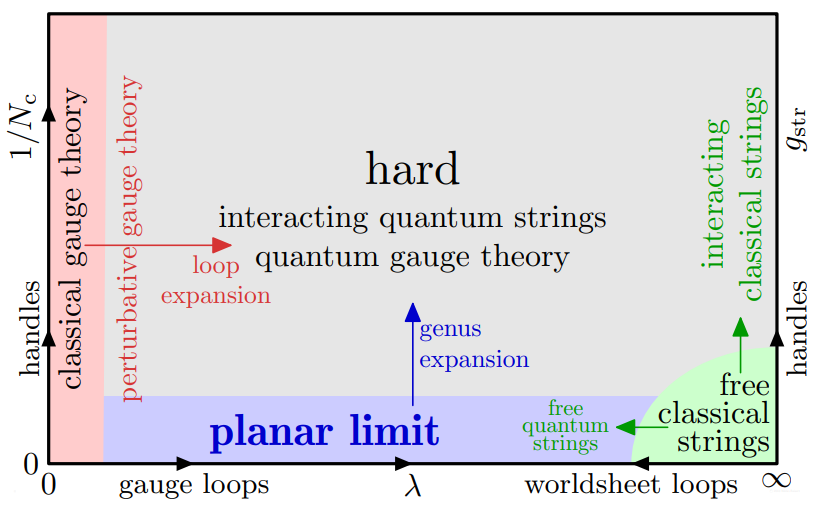
\includegraphics[scale=0.4]{Pictures/N4SYMparameterspace.png}
                \caption{Map of the parameter space of $\mN=4$ SYM or strings on $\text{AdS}_5\times S^5$, from \cite{Beisert_2011}.}
            \end{figure}
            \todo{Explain this diagram.}

        \subsubsection{Moduli space and dynamical phases}

            The scalar potential in \eqref{eq:N4lag} can be written in a rather compact form in terms of the six real scalars $X^i$ making up the three complex scalars $\phi^A$ and reads
            \begin{equation}
                V(X_1,\dots,X_6) = \frac{1}{2}g^2\tr\sum^6_{i,j=1}[X_i,X_j]^2.
            \end{equation}
            The positive definite behavior of the Cartan-Killing form on the compact gauge algebra $\g$ implies that each term in the sum is positive or zero. In other words, $V=0$ is equivalent to
            \begin{equation}
                [X^i,X^j]=0,\qquad i,j=1,\dots,6.
            \end{equation}
            This means that the potential vanishes whenever the scalar fields belong to the Cartan subalgebra of the gauge group $G$. At a generic point of the moduli space, the gauge group is broken to $\U(1)^r$ where $r$ is the rank of $\mathfrak{g}$.
            This equations admit two classes of solutions:
            \begin{itemize}
                \item $\langle X^i\rangle=0$ for all $i=1,\dots,6$. This is the \emph{superconformal phase}. Neither the gauge symmetry nor the superconformal symmetry is broken. The physical states and operators are gauge invariant and transform under
                unitary representations of $\SU(2,2|4)$.
                \item  $\langle X^i\rangle\neq0$ for at least one $i$. This is the \emph{spontaneously broken Coulomb phase}. The gauge algebra $\g$ is going to be broken to $\U(1)^r$, where $r\equiv\rank\g$. The low energy behavior is then the one of $r$ copies of $\mN=4$ $\U(1)$ gauge theories. Superconformal symmetry is spontaneously broken since the non-zero VEV $\langle X^i\rangle$ sets a scale.
            \end{itemize}

            \begin{result}
                \textbf{$\boldsymbol{\mN=4}$ Yang-Mills theory.} There is only one $D=4,\mN=4$ Yang-Mills theory and it contains $3$ $\mN=1$ chiral scalar supermutliplet and $1$ $\mN=1$ vector supermultiplet (up to $g$ and $\tau$). This theory is conformal and can be recovered from dimensional reduction of $D=10,\mN=1$ Yang-Mills on $\mathbb{T}^6$.
            \end{result}
        
    \subsection{Gauge anomaly}\label{sec:anomalies}
        
        The \emph{anomaly degree} $A(\rho)$ of a representation $\rho$ is defined as
        \begin{equation}
            \frac{1}{2}\tr(T_a\{T_b,T_c\})=A(\rho)d_{abc}
        \end{equation}
        where $d_{abc}$ is an invariant symmetric tensor of the Lie algebra of $G$, independent of the representation. One can show that $A(\rho^*)=-A(\rho)$ so self dual representation have $A(\rho)=0$ in particular. The only simple Lie groups that allow for a complex non-self-conjugate representation are $\SU(n)$ with $n\geq3$. We can normalize $d_{abc}$ such that $A(\rho)=1$ for the fundamental $n$-dimensional representations.
    
\section{Properties of D-branes}

    \subsection{SYM from D-branes}

        The dynamics of D-branes is described by the Dirac-Born-Infeld action
        \begin{equation}
            S_{\text{DBI}}[X,F] = -\frac{T_p}{g_s}\int\d^{p+1}\sigma~\sqrt{-\det\limits_{0\leq a,b\leq p}(\eta_{ab}+\p_a X^m\p_b X_m+2\pi\alpha'F_{ab})}.
        \end{equation}
        The latter can be expended for slowly-varying fields, which is equivalent to passing to the field theory limit $\alpha'\to0$. The resulting action is the action of a $\U(1)$ gauge theory in $p+1$ dimensions with $9-p$ real scalar fields. This action is exactly the same than the one we would obtain by dimensionally-reducing a pure $\U(1)$ Yang-Mills gauge theory in 10 spacetime dimensions with the identification
        \begin{equation}
            g_{\text{YM}}=g_sT^{-1}_p(2\pi\alpha')^{-2}=\frac{g_s}{\sqrt{\alpha'}}(2\pi\sqrt{\alpha'})^{p-1}.
        \end{equation}

        This construction can be generalized for multiple D-branes. It now results in a non-abelian theory. The general statement is the following:
        \begin{result}
            The low-energy dynamics of $N$ parallel, coicident D$p$-branes in flat space is described in static gauge by the dimensional reduction to $p+1$ dimensions of pure $10d$ $\mN=1$ supersymmetric Yang-Mills theory with gauge group $\U(N)$ in ten spacetime dimensions.
        \end{result}
        Recall that the $10$-dimensional action is given by
        \begin{equation}
            S_{\text{YM}} = \frac{1}{4g^2_{\text{YM}}}\int\d^{10}x~\left[ \tr(F_{\mu\nu}F^{\mu\nu})+2i\tr(\bar{\psi}\Gamma^\mu D_\mu\psi)\right],\label{eq:SYMaction}
        \end{equation}
        where $F_{\mu\nu}=\p_\mu A_\nu-\p_\nu A_\mu+i[A_\mu,A_\nu]$ is the non-abelian field strength of the $\U(N)$ gauge field $A_\mu$, $D_\mu=\p_\mu-i[A_\mu,\psi]$, $\Gamma^\mu$ are $16\times 16$ Dirac matrices \todo{Why ?}, and the $N\times N$ Hermitian fermion field $\psi$ is a $16$-component Majorana-Weyl spinor of the Lorentz group $\SO(1,9)$ which transforms under the adjoint representation of the gauge group $\U(N)$. On-shell, there are eight on-shell bosonic, gauge field degrees of freedom, and eight fermionic degrees of freedom, after imposition of the Dirac equation $\xout{D}\psi=\Gamma^\mu D_\mu\psi=0$. One can verify that this action is invariant under the supersymmetry transformations
        \begin{align*}
            \delta_\eps A_\mu &= \frac{i}{2}\bar{\eps}\Gamma_\mu\psi,\\
            \delta_{\eps}\psi &= \frac{1}{2}F_{\mu\nu}[\Gamma^\mu,\Gamma^\nu]\eps,
        \end{align*}
        where $\eps$ is an Majorana-Weyl spinor.

        Using \eqref{eq:SYMaction}, we can construct a supersymmetric Yanf-Mills gauge theory in $p+1$ dimensions with $16$ independent supercharges by dimensional reduction: we take all fields to be independent of the coordinates $X^{p+1},\dots, X^9$, then the ten-dimensional gauge field $A_\mu$ splits into a $(p+1)$-dimensional $\U(N)$ gauge field $A_a$ plus $9-p$ Hermitian scalar fields $\Phi^m=X^m/2\pi\alpha'$ in the adjoint representation of $\U(N)$. The D$p$-brane action is thereby obtained from the dimensionality reduced field theory as
        \begin{equation}
            S_{\text{D}p} = -\frac{T_pg_s(2\pi\alpha')^2}{4}\int\d^{p+1}\sigma~\tr\left(F_{ab}F^{ab}+2D_a\Phi^m D^a\Phi_m+\sum_{m\neq n}[\Phi^m,\Phi^n]^2+\text{fermions}\right)\label{eq:SDp}
        \end{equation}
        where $a,b=0,\dots,p$, $m,n=p+1,\dots,9$. We do not explicitly display the fermionic contributions for the moment. In conclusion, the low-energy brane dynamics is described by a supersymmetric Yang-Mills theory on the D$p$-brane worldvolume which is dynamically coupled to the transverse, adjoint scalar fields $\Phi^m$.

        The scalar potential is given by
        \begin{equation}
            V(\Phi)=\sum_{m\neq n}[\Phi^m,\Phi^n]^2.
        \end{equation}
        It is negative definite because $[\Phi^m,\Phi^n]^\dagger=[\Phi^n,\Phi^m]=-[\Phi^m,\Phi^n]$. A classical vacuum of the field theory defined by \eqref{eq:SDp} corresponds to a static solution of the equations of motion whereby the potential energy of the system is minimized. It is given by the field configurations which solve simultaneously the quations $F_{ab}=D_a\Phi^m=\psi^a=0$ and $V(\Phi)=0$. Since all term in $V(\Phi)$ have the same sign, the equation $V(\Phi)=0$ is equivalent to the equation $[\Phi^m,\Phi^n]=0$ for all $m,n$ and at each point in the $(p+1)$-dimensional worldvolume of the branes. This implies that the $N\times N$ hermitian matrix fields $\Phi^m$ are simultaneously diagonalizable by a gauge transformation, so that we may write
        \begin{equation}
            \Phi^m=U
            \begin{bmatrix}
                X^m_1 & & & 0 \\
                & X^m_2 & & \\
                & & \ddots & \\
                0 & & & X^m_N
            \end{bmatrix}U^{-1},\label{eq:diagPhi}
        \end{equation}
        the matrix $U$ is independent of $m$. The simultaneous,
        real eigenvalues $X^m_i$ give the positions of the $N$ distinct D-branes in the $m$-th transverse direction. It follows that the moduli space of classical vacua for the $(p+1)$-dimensional field theory \eqref{eq:SDp} is the quotient space $(\R^{9-p})^N/S_N$, where the factors of $\R$ correspond to the positions of the $N$ D$p$-branes in the $(9-p)$-dimensional transverse space, and $S_N$ is the symmetric group acting by permutations of the $N$ coordinates $X_i$. The group $S_N$ corresponds to the residual Weyl symmetry of the $\U(N)$ gauge group acting in \eqref{eq:diagPhi}. It represents the permutation symmetry of a system of $N$ \emph{indistinguishable} D-branes.

        From \eqref{eq:SDp} one can easily deduce that the masses of the fields corresponding to the off-diagonal matrix elements are given precisely by the distances $\abs{x_i-x_j}$ between the corresponding branes. This description means that an interpretation of the D-brane configuration in terms of classical geometry is only possible in the classical ground state of the system, whereby the matrices $\Phi^m$ are simultaneously diagonalizable and the positions of the individual D-branes may be described through their spectrum of eigenvalues. This gives a simple and natural dynamical mechanism for the appearence of ``non-commutative geometry'' at short distances, where the D-branes cease to have well-defined positions according to classical geometry.

        \todo{The end of this section has to be rewritten}

    \subsection{D-branes and residual SUSY in type II theories}

        The minimal irreducible representation in 10 dimensions is a Majorana-Weyl representation of dimension 8. In type II theories, we have $\mN=(1,1)$ for IIA and $\mN=(2,0)$ for IIB. Because of the string origin of the generators, the two supersymmetry generators $\eps_L$ and $\eps_R$ (Majorana-Weyl spinors) satisfy
        \begin{equation}
            \eps_L=\Gamma_{11}\eps_L,\qquad \eps_R=\eta\Gamma_{11}\eps_R
        \end{equation}
        with $\eta=+1$ for IIB and $\eta=-1$ for IIA theory. For a D$p$-brane, the supersymmetry projections is the following:
        \begin{equation}
            \eps_L=\Gamma_0\dots\Gamma_p\eps_R.
        \end{equation}
        In other words, the supersymmetries with generators of the form
        \begin{equation}
            Q_\alpha+\Gamma_0\dots\Gamma_p\bar{Q}_{\dalpha}\label{eq:susypresved}
        \end{equation}
        are preserved by the D$p$-brane while the one with generators of the form
        \begin{equation}
            Q_\alpha-\Gamma_0\dots\Gamma_p\bar{Q}_{\dalpha}\label{eq:susybroken}
        \end{equation}
        are broken. They violate the boundary conditions. Since there is the same number of generators of the form \eqref{eq:susypresved} than of the form \eqref{eq:susybroken}, exactly haf of the supersymmetry is broken. The idea that one spacetime direction would break one supercharge could be reasonable if supersymmetries were transforming as vectors which not the case; supercharges transform as spinors. It would also be incompatible with the T-duality because two branes of different dimensions must have the same number of unbroken supercharges if there is a T-duality relating them: the number of unbroken supercharges is the same for all dual descriptions (a necessary condition for the equivalence). And indeed, in the correct theory, that's the case. Every type II D-brane breaks half of the supercharges.

        To obtain the previous relations, we start by the ones from M-theory and compactify the 11th direction, getting type IIA theory. $\Gamma_{11}$ then plays the role of the chiral projector in 10 dimensions; the supersymmetry parameters are related by $\eps_L=\frac{1}{2}(1+\Gamma_{11})\eps$ and $\eps_R=\frac{1}{2}(1-\Gamma_{11})\eps$. The relations for type IIB theory are then obtained by T-duality. Under a T-duality over the $\hat{i}$ direction, the supersymmetry parameters transform as
        \begin{align*}
            \eps_L &\mapsto \eps_L,\\
            \eps_R &\mapsto \Gamma_i\eps_R.
        \end{align*}
        The tension of a D$p$-brane is given by
        \begin{equation}
            T_{p} = \frac{1}{(2\pi)^pg_sl^{p+1}_s}.
        \end{equation}
        This completely fixes the Newton constant: the tension of electric-magnetic duals must satisfy:
        \begin{equation}
            T_pT_{D-p-4} = \frac{2\pi}{16\pi G_D}.
        \end{equation}
        In ten dimensions, this gives $G_{10}=8\pi^6g^2_sl^8_s$.

        The dualities are defined as follows:
        \begin{align*}
            \text{S-duality} &: g_s\mapsto\frac{1}{g_s},\qquad l^2_s\mapsto g_sl^2_s,\\
            \text{T-duality} &: R\mapsto\frac{l^2_s}{R},\qquad g\mapsto g_s\frac{l_s}{R}.
        \end{align*}

    \subsection{D-branes wrapping cycles}

        A D$p$-brane worldvolume $\phi:\Sigma\to X$ in spacetime $X$ \emph{wraps} a cycle $c\in H_{p+1}$ if the pushforward $\phi_*(\Sigma)\in H_\text{\textbullet}(X)$ of the fundamental class of $\Sigma$ is the class $[c]$ of the given cycle in $X$. If the pushforward is a mutliple of $[c]$, then the branes wraps $c$ multiple times.

\section{Algebraic geometry}

    \subsection{Elements}

        An important idea in algebraic geometry is that is is really the alegbra of function on it that defines a space. For affine varities $X$, this is illustrated by the fact that the structure of $X$ is really contained in its coordinate ring $K[x_1,\dots,x_n]/I(X)$ and by the isomorphism
        \begin{equation}
            K[x_1,\dots,x_n]|_X=K[x_1,\dots,x_n]/I(X).
        \end{equation}
        Now an algebraic set $Z(T)$ is irreducible if $I(Z(T))$ is prime. So there is a one-to-one correspondence between prime ideals and affine varieties.

        Given an algebraic variety, one can modify the equations continuously by varying some parameters and the variety will be ``deformed'' accordingly. It is called the \emph{variation of the omplex structure}. The space of all complex deformations of an affine variety $X$ is called the \emph{complex moduli space} of $X$. For a Calabi-Yau manifold, the linearization of the complex moduli space (tangent space) is given by the cohomology group $H^{m-1,1}(X)$, where $m$ is the dimension of $X$. In general, it is much more complicated.

    \subsection{Divisors and line bundles}

        A \emph{(Weyl) divisor} $D$ of a complex variety $X$ is a linear combination (formal sum with integer coefficients) of co-dimension one, irreducible subvarieties,
        \begin{equation}
            D=\sum_i n_iV_i,\qquad n_i\in\Z,V_i\subset X.
        \end{equation}
        It said to be effective if all $n_i\geq1$. To any line bundle $L$ with a regular section $s$ (that is, on any open subset $U_\alpha$, $s_\alpha=s|_{U_\alpha}$ is a polyomial in the local coordinates) we can associate a hypersurface $Y\subset X$ defined as
        \begin{equation}
            Y=\{p\in X|s(p)=0\}.
        \end{equation}
        This hypersurface $Y$ can then be decomposed into irreducible parts (affine patches) on which $s_\alpha$ can be factorized in $\C[x_1,\dots,x_n]$ and decomposed in prime ideals $P_i$ of multiplicity $n_i$. Assembling all the $V^\alpha_i$ otgether, we construct co-dimension one subvarities $V_i$ that can be used to form divisors. One can also proceed the other ay around and, given a divisor $D=\sum_i n_iV_i$, define a line bundle $\mathcal{O}_X(D)$ whose sections vanish on each $V_i$ with a zero of order $n_i$. This construction can be generalized to divisors with negative coefficients $n_i<0$ in which case now have poles of order $n_i$ in $V_i$.

    \subsection{Singularities and resolutions}

        A \emph{rational map} from a variety $X$ to another $Y$ is a morphism from a non-empty subset $U\subset X$ to $Y$. Recall that, by definition of the Zariski topology, a non-empty open subset is always dense. Concretely, a rational map can be written in coordinates using ration functions (quotient of polynomials). A \emph{birational map} is an invertible rational map. It induces an isomorphism between two non-empty open subsets. In this case, $X$ and $Y$ are said to be \emph{birationally equivalent}.

        The \emph{resolution of a singularity} of an algebraic variety $V$ is a non-singular variety $W$ with a proper birational map $W\to V$. For varities over fields of characteristic $0$, it was proven (Hironaka, 1964) that \todo{fill in}.

    \subsection{Projective plane curves}

        In $\C\P^2$, we consider a hypersurface defined by a single polynomial $p$ of degree $d$. If
        \begin{equation}
            \pdv{p(x)}{x_i}=0
        \end{equation}
        for all $i$ whenever $p(x)=0$, then the curve is said to be regular, it is a Riemann surface. The latter are classified by their genus and
        \begin{equation}
            g=\frac{(d-1)(d-2)}{2}.
        \end{equation}
        For $d=3$, the most geenral polynomial is
        \begin{equation}
            \sum_{i+j+k=3}c_{ijk}x^i_0x^j_1x^k_2=0
        \end{equation}
        and defines a torus, also called \emph{elliptic curve}. There $10$ independant parameters but $9$ of them can be removed by a $\GL(3,\C)$ transformation, leaving us with only one complex parameter; the complex structrue modulus of the torus.

\section{Quivers representations, path algebras, moduli spaces and quiver varieties}

    \subsection{Quivers, path algebras and relations}

        A quiver $Q$ is a finite directed graph where loops and multiple arrows between edges are allowed. More precisely, it is a piece of combinatorial data $(Q_0,Q_1,t,h)$ such that $Q_0$ is the set of vertice, $Q_1$ the set of arrows and $t,h:Q_1\to Q_0$ are the tail and head maps. A \emph{path} of length $m$ is a trivial composition of arrows $a_1\dots a_m$ such that $h(a_l)=t(a_{l+1})$ for $l=1,\dots,m-1$. It is in particular a \emph{loop} if $h(a_m)=t(a_0)$. We associate to any vertex $i\in Q_0$ a trivial loop $e_i$ going from $i$ to itself. This allows us identify $Q_0$ with the set of paths of lenth $0$. Since $Q_1$ is the set of paths with length $1$ by definition, we can generalize this notation and denote by $Q_m$ be the set of paths of length $m$.
        
        We define the product of paths as
        \begin{equation}
            pq\equiv
            \begin{cases}
                pq,&\quad h(p)=t(q)\\
                0,&\quad\text{else}
            \end{cases}\qquad
            e_ip\equiv
            \begin{cases}
                q,&\quad t(p)=i\\
                0,&\quad\text{else}
            \end{cases}\qquad
            pe_i\equiv
            \begin{cases}
                p,&\quad h(p)=i\\
                0,&\quad\text{else}.
            \end{cases}
        \end{equation}
        We are using the convention that $pq$ means $p$ then $q$. Provided with the formal sum, the set of all paths then forms a ring. Given a field $k$ and an action of $k$ aver this ring we form an algebra, called the \emph{path algebra} of $Q$ and denoted by $kQ$. The addition and multiplication of two elements $a$ and $b$ 
        \begin{equation}
            a=\sum_{\alpha\in Q_m;a_\alpha\in k}\alpha a_\alpha,\qquad b=\sum_{\beta\in Q_m;a_\beta\in k}\beta b_\beta
        \end{equation}
        of $kQ$ are therefore defined as
        \begin{equation}
            a+b=\sum_{\alpha}\alpha(a_\alpha+b_\alpha),\qquad a\cdot b \sum_{\alpha,\beta}\alpha\beta a_\alpha b_\beta.
        \end{equation}
        It is clear that the path algebra is finitely generated if and only if $Q_0$ and $Q_1$ are finite and that it is finite-dimensional if and only if $Q$ has no non-trivial cycles. The $Q_m$'s, the set of paths of length $m$, define a gradation of the path algebra $kQ$:
        \begin{equation}
            kQ=\bigoplus_{m}kQ_m\qquad\text{ with } kQ_m\equiv\bigoplus_{p\in Q_m}pk.
        \end{equation}

        To enforce commutativity of some squares inside a quiver, we can use the notion of relation. A \emph{relation} on a quiver $Q$ is a $k$-linear combination of paths from $Q$. More precisely, is a subsapce of $kQ$ spanned by linear combinations of paths having a common source and common target, and of length at least $2$. A \emph{quiver with relations} is a pair $(Q,I(R))$ where $I(R)\subseteq kQ$ is the (two-sided) ideal of the path algebra generated by $R$. The path algebra of $(Q,I)$ is $kQ/I(R)$. 
        
        \begin{examp*}
            If $Q$ is the $r$-loop, then a relation is a subspace of $kQ = k\langle X_1,\dots,X_r\rangle$ spanned by linear combinations of words of length at least 2. For instance, all the commutators $X_iX_j-X_jX_i$, then the two elements of $kQ$ correspond to the same element in $kQ/I(R)$ if and only their difference is in $I(R)$. In this case, this means that they only differ by inverting the product of two variables in their expression. The resulting algebra is then the ``commutative version'' of $kQ$, which is nothing but than the polynomial algebra $k[X_1,\dots,X_r]$.
        \end{examp*}

    \subsection{Quiver representations}

        A \emph{representation} of a quiver $Q$ over the field $k$ is an assignment to every vertex $i$ os a $k$-vector space $V_i$ and to every arrow $a$ a linear mapping $f_a=V_{t(a)}\to V_{h(a)}$ between the corresponding vector spaces to each arrow. A representation of a quiver with relations $(Q,R)$ has the same definition but with the additional requirement that the linear maps must preserve the relations. \todo{Explain.} Denoting $\alpha_i=\dim V_i$, $\alpha=(\alpha_i)\in\N^{Q_0}_0$ is the \emph{dimension vector} of the representation. Quiver representations are an effective combinatorial tool for organizing linear algebraic data. Not only are they naturally related to many algebraic objects such as quantum groups, Kac-Moody algebras, and cluster algebras, but they have also been studied from the geometric point of view, often serving to bridge the gap between representation theory and algebraic geometry. 
        
        If $V=(V_i,f_a)$ and $W=(W_i,g_a)$ are are two finite-dimensional representation of the same quiver with relations $(Q,R)$, a morphism $\psi$ from $V$ to $W$ is given by specifying , for every vertex $i$, a linear isomorphism $\psi_i:V_i\to W_i$ such that for avery arrow $a$ $\psi_{h(a)}\circ f_a=g_a\circ\psi_{t(a)}$. The \emph{direct sum} $V\oplus W$ of representations can also be defined as $(V\oplus W)_i=V_i\oplus W_i$ with the direct sum of the linear mappings. We then say that a representation is \emph{decomposable} is it is isomorphic to the direct sum of non-zero representations and of \emph{finite-type} (or \emph{finite orbit type}) if it has only finitely many isomorphism classes of indecomposable representations. Or, equivalently, if it has only finitely many isomorphism classes of representations for any prescribed dimension vector. A very important theorem in indecomposable representations is the following:
        \begin{theorem*}[Gabriel]
            A (connected) quiver is of fnite type if and only if its underlying undirected graph is a simply-laced Dynkin diagram.
        \end{theorem*}
        
        To any representation $V=(V_i,f_a)$ of $Q$ we can associate a $k$-vector space
        \begin{equation}
            V=\bigoplus_{i \in Q_0}V_i
        \end{equation}
        equipped with two famillies of linear self-maps: the projections $f_i:V\to V$ ($i\in Q_0$) obtained from the composition $V\hookrightarrow V_i\to V$ of the projections with the inclisions, and tha maps $f_a:V\to V$ ($a\in Q_1$) obtained similarly from the defining maps $f_a=V_{t(a)\to V_{h(a)}}$. One can see that these maps satisfy the relations
        \begin{equation}
            f^2_i=f_i,\qquad f_i\circ f_j=0~(i\neq j),\qquad f_{t(a)}\circ f_a=f_a\circ f_{h(a)}=f_a
        \end{equation}
        and all other products are zero. In this sense, representations a quiver defines an algebra (the algebra of $f_i$ and $f_a$). Now comes the whole point to all this is: this algebra is a representation of the path algebra. To see this, we can use the notation $\rho(e_i)=f_i:V\to V$ and $\rho(a)=f_a:V\to V$ so $\rho:kQ\to \End(V)$ and we can show that is is a $k$-linear morphism of rings. So $\rho$ is a representation of the algebra $kQ$. So a representation of a quiver $Q$ gives a representation of the path algebra. Conversely, given the path algebra $kQ$ of a quiver, then $kQ$ is in particular a vector space over $k$ that yields a familly of vector space $\{V_i=e_i V\}_{i\in Q_0}$ and we have a linear map $f_a:V_{t(a)}\to V_{h(a)}$ for any arrow $a\in Q_1$. We conclude that representations of the path algebra and of the quiver are equivalent. Gabriel's theorem could then be equivalently phrased as: the path algebra of any quiver has finite representations if and only if it is ADE.
        
        Recall also that giving a $k$-linear morphism $A=(k,R)\to\End(V)$ is equivalent to giving a structure of $R$-module to $V$. So from what we discussed above, giving a representation of a quiver is equivalent to giving a module structure to $V$. This can be rephrased using a more categorical language by showing that these constructions extend to functors. It is now clear that the finite-dimensional representations of a quiver with relations form a category, which we denote by $\texttt{fRep}(kQ,R)$. If $(Q,I(R))$ is a quiver with relations and $A=kQ/I$ its path algebra, then the set of finite-dimensional modules of $A$ is also a category that we denote by $\texttt{fdmod}A$. There is a categorical equivalence
        \begin{equation}
            \boxed{\texttt{fRep}(kQ,R)\approx\texttt{fdmod}A.}
        \end{equation}

        The representation of any finite-dimensional alegbra can be described by a quiver with relations $(Q,I)$ such that $I$ contains the power of the ideal generated by the arrows.

    \subsection{Geometric invariant theory}

    \subsection{GIT quotient for quiver representation}

    \subsection{Quiver varities}

    \subsection{Moduli problems}

        Given a collection of algebra-geometric objects it is natural to try to classify these objects up to equivalence. Naively, given a collection $\A$ of such objects and an equivalence relation $\sim$ on $\A$, one may ask whether there exists an algebraic variety $X$ whose points (over the base field $k$) correspond to equivalence classes in $\A/\sim$. This approach is flawed, since there may be many such varieties and some are better than others at retaining the relationships between the objects being classified. If, for example, we are interested in classifying all lines through the origin in the complex plane $\C^2$ up to equality, we can view the corresponding equivalence classes as points of the complex projective line $\P^1_\C$, but we can also see them as points in the disjoint union $\bbA^1_\C\sqcup\{pt\}$ of a line and a point. Ideally, the points of the variety solving a moduli problem should be configured to reflect the relationship between the geometric objects they parametrize.
        
        Thus, in more nuanced approach we try to describe equivalence classes of families of objects of $\A$, rather than just of the objects themselves. That is, we look at pairs $\F,T$, consisting of a variety $T$ and a family $\pi:\F\to X$ of objects of $\A$ (the fibers $\pi^{-1}(t)$ are objects of $\A$) subject to some additional conditions (e.g. that $\pi$ is flat). Moreover, if the collection of families over a variety $T$ is denoted by $\A_T$, then for any morphism $f:S\to T$, there should be a pullback operation assigning to any family $\F\in \A_T$ a family $f^*\F\in\A_S$. Now, we can extend our moduli problem by introducing an equivalence relation $\sim_T$ on $A_T$ that is compatible with pullback and give us the starting equivalence relation $\sim$ when $T$ is $\text{Spec}k$.
        
        The solution to such an extended moduli problem, called a \emph{fine moduli space}, consists of a variety $X$ whose $k$-points classify equivalence classes in $\A/\sim$, together with a \emph{universal family} $\mathcal{U}\in\A_X$, which describes how these equivalence classes relate to each other. More specifically, any family $\F\in\A_T$ over a variety $T$ is equivalent to the pullback $f^*\mathcal{U}$ along a unique morphism $f:T\to X$. In the special case that $T=\text{Spec}k$, we obtain that the $k$-points of $X$ are in bijection with equivalence classes in $\A$. Furthermore, it turns out that the fine moduli space is
        unique up to isomorphism. 
        
        Considering once again the example of lines through the origin in $\C^2$, we see that a family of such lines over a variety $T$ may be thought of as a line subbundle $\mathcal{L}\subset\C^2\times T\to T$ of the trivial rank $2$ vector bundle over $T$. The equivalence relation becomes an isomorphism of line subbundles of $\C^2\times T$. The solution to the corresponding moduli problem consists of the complex projective line $\P^1_\C$ together with the tautological line bundle $\mathcal{O}_{\P^1_\C}(-1)$. Indeed, if $\mathcal{L}\subset\C^2\times T$ is a subbundle, then its dual $\mathcal{L}^\vee$ is generated by global sections (specifically, the images of the standard global sections with respect to the surjection   $(\C^2)^\vee\times T\twoheadrightarrow\mathcal{L}^\vee)$. This defines a unique morphism $f:T\to\P^1_\C$ such that $\mathcal{L}\simeq f^*\mathcal{O}(-1)$.

        Unfortunately, it is often the case that, for a given class of objects $\A$, a fine modduli space either does not exist or requires us to place restrictions on the kinds of objects in $\A$ we wish to classify. In order to avoid this, we can forget the universal family and look for a nice enough variety with points in bijection with equivalence classes in $\A/\sim$. Alternatively, we can allow for the solution of our moduli problem to no longer be a variety (or even a scheme). The result is a more complicated object called a \emph{stack}.


    \todo{This section has to be rewritten.}

\section{Quivers in string theory and Yang-mills in graph theory}

\section{Calabi-Yau manifolds, orbifolds and crepant resolutions}\label{sec:CY}

    \subsection{Kähler, Calabi-Yau structure and moduli spaces}

        The Kähler form $\omega$ is a representative of a Doleault cohomology class
        \begin{equation}
            [\omega]\in H^{1,1}(X)
        \end{equation}
        and $[\omega]$ is called the \emph{Hähler class} of $\omega$.
        \begin{theorem}[Calabi-Yau]
            Given $X$ a compact manifold with trivial canonical bundle, and given a Kähler form $\tilde{\omega}$ on $X$, there exist a unique Ricci-flat metric in the Kähler class of $\tilde{\omega}$. That is, a unique Ricci-flat metric defined for some $\omega\in[\tilde{\omega}]$.
        \end{theorem}
        On the other hand, it is easy to show that Ricci-flatness implies triviality of the canonical bundle. For non-compact manifolds, the theorem does not hold strictly speaking, one must specify boundary conditions at infinity to find a Ricci-flat metric.

        Given a Calabi-Yau anifold, we see that there are continuous famillies of Ricci-flat metrics, one for each cohomology class of $H^{1,1}(X)$. One can decompose any chomology class on a basis $[\omega]^i$ of the vactor space $H^{1,1}(X)$
        \begin{equation}
            [\omega]=\sum^{h^{1,1}}_{i=1}\lambda_i[\omega]^i.
        \end{equation}
        It is called the \emph{Kähler moduli space} of $X$ and its dimension is denoed by $h^{1,1}$.

    \subsection{Calabi-Yau manifolds}

        A \emph{Calabi-Yau manifold} of (complex) dimension $n$ is a compact $n$-dimensional Kähler manifold $M$ satisfying one of the following equivalent conditions:
        \begin{itemize}
            \item the canonical bundle of $M$ is trivial,
            \item $M$ has holomorphic $n$-form that vanishes nowhere,
            \item the structure group of the tangent bundle of $M$ can be reduced from $\U(n)$ to $\SU(n)$,
            \item $M$ has Kähler metric with global holonomy contained in $\SU(n)$.
        \end{itemize}

        It was conjectured by Calabi then prooved by Yau that such spaces are necessarily Ricci-flat. In particular, since the first Chern class of CY manifolds si given by
        \begin{equation}
            c_1=\frac{1}{2\pi}[\mathcal{R}]
        \end{equation}
        it implies that $c_1$ vanishes, the converse is not true.

        For a compact $n$-dimensioanl Kähler manifold the following conditions are equivalent to each other:
        \begin{itemize}
            \item the first real Chern class vanishes,
            \item $M$ has a Kähler metric with vanishing Ricci curvature,
            \item $M$ has Kähler metric with local holonomy contained in $\SU(n)$.
            \item a positive power of the canonical bundle of $M$ is trivial,
            \item $M$ has a finite cover that has trivial canonical bundle,
            \item $M$ has a finite cover that is a product of a torus and a simply connected manifold with trivial canonical bundle.
        \end{itemize}
        They are weaker than the conditions above except when the Kähler manifold is simply connected in which case they are equivalent.

    \subsection{Calabi-Yau orbifolds}

        A \emph{Calabi-Yau orbifold} is the quotient of a smooth Calabi-Yau manifold by a discrete group action which generically has fixed points. From a algebraic geometry perspective we can try to resolve the orbifold singularity. A resolution $(X,\pi)$ of $\C^n/\Gamma$ is a non-singular complex manifold $X$ of dimension $n$ with a proper biholomorphic map 
        \begin{equation}
            \pi:X\to\C^n/\Gamma
        \end{equation}
        that induces a biholomorphism between dense open sets. A resolution $(X,\pi)$ of $\C^n/\Gamma$ is called a \emph{crepant resolution}\index{resolution!crepant}\footnote{For a resolution of singularities we can define a notion of discrepancy. A crepant resolution is a resolution
            without discrepancy.} if the canonical bundles of $X$ and $\C^n/\Gamma$ are isomorphic, i.e.
            \begin{equation*}
                K_X\cong\pi^*(K_{\C^n/\Gamma}).
            \end{equation*}
        Since Calabi-Yau manifolds have trivial canonical bundle, to obtain a Calabi-Yau structure on $X$ one must choose a crepant resolutions of singularities.

        It turns out that the amount of information we know about a crepant resolution of singularities of $\C^n/\Gamma$ depends dramatically on the dimension $n$ of the orbifold:
        \begin{itemize}
            \item $n=2$: a crepant always exists and is unique. Its topology is entirely described in terms of the finite group $\Gamma$ (via the McKay correspondence).
            \item $n=3$: a crepant resolution always exists but it is not unique; they are related by flops. However all the crepant resolutions have the same Euler and Betti numbers: the \emph{stringy} Betti and Hodge numbers of the orbifold.
            \item $n\geq4$: very little is known; crepant resolution ecists in rather special cases. Many singularity are terminal, which implies that they admit no crepant resolution.
        \end{itemize}

\section{McKay correspondence}\label{app:McKay}

    \subsection{Classical correspondence}

        \begin{table}[H]
            \centering
            \begin{tabular}{|c|l|l|l|}
                \hline
                $\Gamma\subset\SU(2)$ & Platonic solids & McKay graph & Algebraic variety \\ \hline
                $\Z_n$ &  & \begin{tikzpicture}[baseline={($ (current bounding box.center) - (0,3pt) $)},scale=0.5]
                    \draw (0,0) edge (2*1.25,0);
                    \draw (2*1.25,0) edge[dashed] (3*1.25,0);
                    \draw (3*1.25,0) edge (4*1.25,0);
                    \draw (0,0) edge (2*1.25,-1);
                    \draw (4*1.25,0) edge (2*1.25,-1);
                    \foreach \x in {0,1,2,3,4} {
                        \draw[fill=black] (1.25*\x,0) circle[radius=0.15];
                        \draw (1.25*\x,0) node[above]{$1$};
                    }
                    \draw[fill=black] (1.25*2,-1) circle[radius=0.15];
                    \draw (1.25*2,-1) node[above]{$1$};
                \end{tikzpicture}\quad($n$ nodes) & $z^{n}+xy=0$ \\ \hline
                $2\mathcal{D}_n$ & $n$-polygon & \begin{tikzpicture}[baseline={($ (current bounding box.center) - (0,3pt) $)},scale=0.5]
                    \draw (0,0) edge (2*1.25,0);
                    \draw (2*1.25,0) edge[dashed] (3*1.25,0);
                    \draw (3*1.25,0) edge (4*1.25,0);
                    \draw (4*1.25,0) edge (5*1.25,0);
                    \draw (1.25,0) edge (1.25,-1.25);
                    \draw (4*1.25,0) edge (4*1.25,-1.25);
                    \foreach \x in {0,1,2,3,4,5} {
                        \draw[fill=black] (1.25*\x,0) circle[radius=0.15];
                    }
                    
                    \draw[fill=black] (1.25,-1.25) circle[radius=0.15];
                    \draw (1.25,-1.25) node[right]{$1$};
                    \draw[fill=black] (4*1.25,-1.25) circle[radius=0.15];
                    \draw (4*1.25,-1.25) node[right]{$1$};
                    \draw (0,0) node[above]{$1$};
                    \draw (1.25*5,0) node[above]{$1$};
                    \draw (1.25*1,0) node[above]{$2$};
                    \draw (1.25*2,0) node[above]{$2$};
                    \draw (1.25*3,0) node[above]{$2$};
                    \draw (1.25*4,0) node[above]{$2$};
                \end{tikzpicture}\quad($n+3$ nodes) & $x^2+y^2z+z^{n-1}=0$ \\ \hline
                $2\mathcal{T}$ & tetrahedron & \begin{tikzpicture}[baseline={($ (current bounding box.center) - (0,3pt) $)},scale=0.5]
                    \draw (0,0) edge (4*1.25,0);
                    \draw (2*1.25,0) edge (2*1.25,-2*1.25);
                    \foreach \x in {0,1,2,3,4} {
                        \draw[fill=black] (1.25*\x,0) circle[radius=0.15];
                    }
                    \draw[fill=black] (2*1.25,-1.25) circle[radius=0.15];
                    \draw (2*1.25,-1.25) node[right]{$2$};
                    \draw[fill=black] (2*1.25,-2*1.25) circle[radius=0.15];
                    \draw (2*1.25,-2*1.25) node[right]{$1$};
                    \draw (0,0) node[above]{$1$};
                    \draw (1.25*4,0) node[above]{$1$};
                    \draw (1.25*1,0) node[above]{$2$};
                    \draw (1.25*2,0) node[above]{$3$};
                    \draw (1.25*3,0) node[above]{$2$};
                \end{tikzpicture}\quad($7$ nodes) & $x^2+y^3+z^4=0$ \\ \hline
                $2\mathcal{O}$  & \begin{tabular}{@{}l@{}}cube \\ octahedron\end{tabular} & \begin{tikzpicture}[baseline={($ (current bounding box.center) - (0,3pt) $)},scale=0.5]
                    \draw (0,0) edge (6*1.25,0);
                    \draw (3*1.25,0) edge (3*1.25,-1.25);
                    \foreach \x in {0,1,2,3,4,5,6} {
                        \draw[fill=black] (1.25*\x,0) circle[radius=0.15];
                    }
                    \draw[fill=black] (3*1.25,-1.25) circle[radius=0.15];
                    \draw (3*1.25,-1.25) node[right]{$2$};
                    \draw (0,0) node[above]{$1$};
                    \draw (1.25*1,0) node[above]{$2$};
                    \draw (1.25*2,0) node[above]{$3$};
                    \draw (1.25*3,0) node[above]{$4$};
                    \draw (1.25*4,0) node[above]{$3$};
                    \draw (1.25*5,0) node[above]{$2$};
                    \draw (1.25*6,0) node[above]{$1$};
                \end{tikzpicture}\quad($8$ nodes) & $x^2+y^3+yz^3=0$ \\ \hline
                $2\mathcal{I}$  & \begin{tabular}{@{}l@{}}icosahedron \\ dodecahedron\end{tabular} & \begin{tikzpicture}[baseline={($ (current bounding box.center) - (0,3pt) $)},scale=0.5]
                    \draw (0,0) edge (7*1.25,0);
                    \draw (2*1.25,0) edge (2*1.25,-1.25);
                    \foreach \x in {0,1,2,3,4,5,6,7} {
                        \draw[fill=black] (1.25*\x,0) circle[radius=0.15];
                    }
                    \draw[fill=black] (2*1.25,-1.25) circle[radius=0.15];
                    \draw (2*1.25,-1.25) node[right]{$3$};
                    \draw (0,0) node[above]{$2$};
                    \draw (1.25*1,0) node[above]{$4$};
                    \draw (1.25*2,0) node[above]{$6$};
                    \draw (1.25*3,0) node[above]{$5$};
                    \draw (1.25*4,0) node[above]{$4$};
                    \draw (1.25*5,0) node[above]{$3$};
                    \draw (1.25*6,0) node[above]{$2$};
                    \draw (1.25*7,0) node[above]{$1$};
                \end{tikzpicture}\quad($9$ nodes) & $x^2+y^3+z^5=0$ \\ \hline
            \end{tabular}
            \caption{Binary polyhedral groups and their McKay graphs.Labels over the vertices are the dimension of the representation. We erase the arrow ends if they go in both directions and erase the label if it is
            equal to $1$.}
        \end{table}

        \begin{figure}[H]
            \centering
            \begin{tabular}{|c|c|l|}
                \hline
                \begin{tabular}{@{}c@{}}Simple \\ Lie algebra\end{tabular} & Simply laced & \begin{tabular}{@{}l@{}}Dynkin diagram \\ Extended Dybkin diagram\end{tabular} \\ \hline
                $\mathfrak{sl}(n+1,\C),n\geq1$ & yes & 
                \begin{tabular}{@{}l@{}} $A_n:\quad$ \begin{tikzpicture}[baseline={($ (current bounding box.center) - (0,3pt) $)},scale=0.5]
                    \draw (0,0) edge (2*1.25,0);
                    \draw (2*1.25,0) edge[dashed] (3*1.25,0);
                    \draw (3*1.25,0) edge (4*1.25,0);
                    \foreach \x in {0,1,2,3,4} {
                    \draw[fill=white] (1.25*\x,0) circle[radius=0.15];
                    }
                    \end{tikzpicture}\quad($n$ nodes) \\[0.4cm] $\tilde{A}_n:\quad$ \begin{tikzpicture}[baseline={($ (current bounding box.center) - (0,3pt) $)},scale=0.5]
                        \draw (0,0) edge (2*1.25,0);
                        \draw (2*1.25,0) edge[dashed] (3*1.25,0);
                        \draw (3*1.25,0) edge (4*1.25,0);
                        \draw (0,0) edge (2*1.25,1);
                        \draw (4*1.25,0) edge (2*1.25,1);
                        \foreach \x in {0,1,2,3,4} {
                            \draw[fill=white] (1.25*\x,0) circle[radius=0.15];
                        }
                        \draw[fill=black] (1.25*2,1) circle[radius=0.15];
                    \end{tikzpicture}\quad($n+1$ nodes)\end{tabular} \\ \hline
                $\mathfrak{so}(2n+1,\R),n\geq2$ & no & 
                \begin{tabular}{@{}l@{}}$B_n:\quad$ \begin{tikzpicture}[baseline={($ (current bounding box.center) - (0,3pt) $)},scale=0.5]
                    \draw (0,0) edge (2*1.25,0);
                    \draw (2*1.25,0) edge[dashed] (3*1.25,0);
                    \draw (3*1.25+0.65-0.15,0.21) -- (3*1.25+0.65+0.15,0) -- (3*1.25+0.65-0.15,-0.21);
                    \draw (3*1.25,0.07) -- (4*1.25,0.07);
                    \draw (3*1.25,-0.07) -- (4*1.25,-0.07); 
                    \foreach \x in {0,1,2,3,4} {
                    \draw[fill=white] (1.25*\x,0) circle[radius=0.15];
                    }
                    \end{tikzpicture}\quad ($n$ nodes) \\[0.4cm] $\tilde{B}_n:\quad$ \begin{tikzpicture}[baseline={($ (current bounding box.center) - (0,3pt) $)},scale=0.5]
                        \draw (1.25,0) edge (2*1.25,0);
                        \draw (0,0.7) edge (1.25,0);
                        \draw (0,-0.7) edge (1.25,0);
                        \draw (2*1.25,0) edge[dashed] (3*1.25,0);
                        \draw (3*1.25+0.65-0.15,0.21) -- (3*1.25+0.65+0.15,0) -- (3*1.25+0.65-0.15,-0.21);
                        \draw (3*1.25,0.07) -- (4*1.25,0.07);
                        \draw (3*1.25,-0.07) -- (4*1.25,-0.07); 
                        \foreach \x in {1,2,3,4} {
                            \draw[fill=white] (1.25*\x,0) circle[radius=0.15];
                        }
                        \draw[fill=white] (0,0.7) circle[radius=0.15];
                        \draw[fill=black] (0,-0.7) circle[radius=0.15];
                    \end{tikzpicture}\quad($n+1$ nodes)\end{tabular} \\ \hline
                $\mathfrak{sp}(2n,\C),n\geq3$ & no & 
                \begin{tabular}{@{}l@{}}$C_n:\quad$ \begin{tikzpicture}[baseline={($ (current bounding box.center) - (0,4pt) $)},scale=0.5]
                    \draw (0,0) edge (2*1.25,0);
                    \draw (2*1.25,0) edge[dashed] (3*1.25,0);
                    \draw (3*1.25+0.65+0.15,0.21) -- (3*1.25+0.65-0.15,0) -- (3*1.25+0.65+0.15,-0.21);
                    \draw (3*1.25,0.07) -- (4*1.25,0.07);
                    \draw (3*1.25,-0.07) -- (4*1.25,-0.07); 
                    \foreach \x in {0,1,2,3,4} {
                    \draw[fill=white] (1.25*\x,0) circle[radius=0.15];
                    }
                    \end{tikzpicture}\quad ($n$ nodes) \\[0.4cm] $\tilde{C}_n:\quad$ \begin{tikzpicture}[baseline={($ (current bounding box.center) - (0,4pt) $)},scale=0.5]
                        \draw (0.65-0.15,0.21) -- (0.65+0.15,0) -- (0.65-0.15,-0.21);
                        \draw (0,0.07) -- (1.25,0.07);
                        \draw (0,-0.07) -- (1.25,-0.07);
                        \draw (1.25,0) edge (2*1.25,0);
                        \draw (2*1.25,0) edge[dashed] (3*1.25,0);
                        \draw (3*1.25+0.65+0.15,0.21) -- (3*1.25+0.65-0.15,0) -- (3*1.25+0.65+0.15,-0.21);
                        \draw (3*1.25,0.07) -- (4*1.25,0.07);
                        \draw (3*1.25,-0.07) -- (4*1.25,-0.07); 
                        \foreach \x in {1,2,3,4} {
                            \draw[fill=white] (1.25*\x,0) circle[radius=0.15];
                        }
                        \draw[fill=black] (0,0) circle[radius=0.15];
                    \end{tikzpicture}\quad($n+1$ nodes)\end{tabular} \\ \hline
                $\mathfrak{so}(2n,\R),n\geq4$ & yes &
                \begin{tabular}{@{}l@{}}$D_n:\quad$ \begin{tikzpicture}[baseline={($ (current bounding box.center) - (0,3pt) $)},scale=0.5]
                    \draw (0,0) edge (2*1.25,0);
                    \draw (2*1.25,0) edge[dashed] (3*1.25,0);
                    \draw (3*1.25,0) -- (4*1.25,0.7);
                    \draw (3*1.25,0) -- (4*1.25,-0.7); 
                    \foreach \x in {0,1,2,3} {
                    \draw[fill=white] (1.25*\x,0) circle[radius=0.15];
                    }
                    \draw[fill=white] (1.25*4,0.7) circle[radius=0.15];
                    \draw[fill=white] (1.25*4,-0.7) circle[radius=0.15];
                    \end{tikzpicture}\quad($n$ nodes) \\[0.4cm] $\tilde{D}_n:\quad$  \begin{tikzpicture}[baseline={($ (current bounding box.center) - (0,3pt) $)},scale=0.5]
                        \draw (0,0.7) edge (1.25,0);
                        \draw (0,-0.7) edge (1.25,0);
                        \draw (1.25,0) edge (2*1.25,0);
                        \draw (2*1.25,0) edge[dashed] (3*1.25,0);
                        \draw (3*1.25,0) -- (4*1.25,0.7);
                        \draw (3*1.25,0) -- (4*1.25,-0.7); 
                        \foreach \x in {1,2,3} {
                            \draw[fill=white] (1.25*\x,0) circle[radius=0.15];
                        }
                        \draw[fill=white] (0,0.7) circle[radius=0.15];
                        \draw[fill=black] (0,-0.7) circle[radius=0.15];
                        \draw[fill=white] (1.25*4,0.7) circle[radius=0.15];
                        \draw[fill=white] (1.25*4,-0.7) circle[radius=0.15];
                    \end{tikzpicture}\quad($n+1$ nodes)\end{tabular} \\ \hline
                $\mathfrak{e}_6$ & yes &
                \begin{tabular}{@{}l@{}}$E_6:\quad$ \begin{tikzpicture}[baseline={($ (current bounding box.south) + (0,1pt) $)},scale=0.5]
                    \draw (0,0) edge (4*1.25,0);
                    \draw (2*1.25,0) edge (2*1.25,1.25);
                    \foreach \x in {0,1,2,3,4} {
                    \draw[fill=white] (1.25*\x,0) circle[radius=0.15];
                    }
                    \draw[fill=white] (2*1.25,1.25) circle[radius=0.15];
                    \end{tikzpicture} \quad($6$ nodes) \\[0.4cm]  $\tilde{E}_6:\quad$ \begin{tikzpicture}[baseline={($ (current bounding box.south) + (0,1pt) $)},scale=0.5]
                        \draw (0,0) edge (4*1.25,0);
                        \draw (2*1.25,0) edge (2*1.25,2*1.25);
                        \foreach \x in {0,1,2,3,4} {
                            \draw[fill=white] (1.25*\x,0) circle[radius=0.15];
                        }
                        \draw[fill=white] (2*1.25,1.25) circle[radius=0.15];
                        \draw[fill=black] (2*1.25,2*1.25) circle[radius=0.15];
                    \end{tikzpicture}\quad($7$ nodes)\end{tabular} \\ \hline
                $\mathfrak{e}_7$ & yes & 
                \begin{tabular}{@{}l@{}} $E_7:\quad$ \begin{tikzpicture}[baseline={($ (current bounding box.south) + (0,1pt) $)},scale=0.5]
                    \draw (0,0) edge (5*1.25,0);
                    \draw (2*1.25,0) edge (2*1.25,1.25);
                    \foreach \x in {0,1,2,3,4,5} {
                    \draw[fill=white] (1.25*\x,0) circle[radius=0.15];
                    }
                    \draw[fill=white] (2*1.25,1.25) circle[radius=0.15];
                    \end{tikzpicture} \quad($7$ nodes) \\[0.4cm] $\tilde{E}_7:\quad$ \begin{tikzpicture}[baseline={($ (current bounding box.south) + (0,1pt) $)},scale=0.5]
                        \draw (-1.25,0) edge (5*1.25,0);
                        \draw (2*1.25,0) edge (2*1.25,1.25);
                        \foreach \x in {0,1,2,3,4,5} {
                            \draw[fill=white] (1.25*\x,0) circle[radius=0.15];
                        }
                        \draw[fill=black] (-1.25,0) circle[radius=0.15];
                        \draw[fill=white] (2*1.25,1.25) circle[radius=0.15];
                    \end{tikzpicture}\quad($8$ nodes)\end{tabular} \\ \hline
                $\mathfrak{e}_8$ & yes & 
                \begin{tabular}{@{}l@{}}$E_8:\quad$ \begin{tikzpicture}[baseline={($ (current bounding box.south) + (0,1pt) $)},scale=0.5]
                    \draw (0,0) edge (6*1.25,0);
                    \draw (2*1.25,0) edge (2*1.25,1.25);
                    \foreach \x in {0,1,2,3,4,5,6} {
                    \draw[fill=white] (1.25*\x,0) circle[radius=0.15];
                    }
                    \draw[fill=white] (2*1.25,1.25) circle[radius=0.15];
                    \end{tikzpicture} \quad($8$ nodes) \\[0.4cm] $\tilde{E}_8:\quad$ \begin{tikzpicture}[baseline={($ (current bounding box.south) + (0,1pt) $)},scale=0.5]
                        \draw (0,0) edge (7*1.25,0);
                        \draw (2*1.25,0) edge (2*1.25,1.25);
                        \foreach \x in {0,1,2,3,4,5,6} {
                            \draw[fill=white] (1.25*\x,0) circle[radius=0.15];
                        }
                        \draw[fill=black] (7*1.25,0) circle[radius=0.15];
                        \draw[fill=white] (2*1.25,1.25) circle[radius=0.15];
                    \end{tikzpicture}\quad($9$ nodes)\end{tabular} \\ \hline
                $\mathfrak{f}_4$ & no & 
                \begin{tabular}{@{}l@{}}$F_4:\quad$ \begin{tikzpicture}[baseline={($ (current bounding box.center) - (0,3pt) $)},scale=0.5]
                    \draw (0,0) edge (1.25,0);
                    \draw (2*1.25,0) edge (3*1.25,0);
                    \draw (1*1.25+0.65-0.15,0.21) -- (1*1.25+0.65+0.15,0) -- (1*1.25+0.65-0.15,-0.21);
                    \draw (1*1.25,0.07) -- (2*1.25,0.07);
                    \draw (1*1.25,-0.07) -- (2*1.25,-0.07); 
                    \foreach \x in {0,1,2,3} {
                    \draw[fill=white] (1.25*\x,0) circle[radius=0.15];
                    }
                    \end{tikzpicture} \quad($4$ nodes) \\[0.4cm] $\tilde{F}_4:\quad$  \begin{tikzpicture}[baseline={($ (current bounding box.center) - (0,3pt) $)},scale=0.5]
                        \draw (-1.25,0) edge (1.25,0);
                        \draw (2*1.25,0) edge (3*1.25,0);
                        \draw (1*1.25+0.65-0.15,0.21) -- (1*1.25+0.65+0.15,0) -- (1*1.25+0.65-0.15,-0.21);
                        \draw (1*1.25,0.07) -- (2*1.25,0.07);
                        \draw (1*1.25,-0.07) -- (2*1.25,-0.07); 
                        \foreach \x in {0,1,2,3} {
                            \draw[fill=white] (1.25*\x,0) circle[radius=0.15];
                        }
                        \draw[fill=black] (-1.25,0) circle[radius=0.15];
                    \end{tikzpicture}\quad($5$ nodes)\end{tabular} \\ \hline
                $\mathfrak{g}_2$ & no & 
                \begin{tabular}{@{}l@{}} $G_2:\quad$  \begin{tikzpicture}[baseline={($ (current bounding box.center) - (0,3pt) $)},scale=0.5]
                    \draw (0,0) edge (1.25,0);
                    \draw (0.65-0.15,0.21) -- (0.65+0.15,0) -- (0.65-0.15,-0.21);
                    \draw (0,0.11) -- (1.25,0.11);
                    \draw (0,-0.11) -- (1.25,-0.11); 
                    \foreach \x in {0,1} {
                    \draw[fill=white] (1.25*\x,0) circle[radius=0.15];
                    }
                    \end{tikzpicture} \quad($2$ nodes) \\[0.4cm] $\tilde{G}_2:\quad$ \begin{tikzpicture}[baseline={($ (current bounding box.center) - (0,3pt) $)},scale=0.5]
                        \draw (-1.25,0) edge (1.25,0);
                        \draw (0.65-0.15,0.21) -- (0.65+0.15,0) -- (0.65-0.15,-0.21);
                        \draw (0,0.11) -- (1.25,0.11);
                        \draw (0,-0.11) -- (1.25,-0.11); 
                        \foreach \x in {0,1} {
                            \draw[fill=white] (1.25*\x,0) circle[radius=0.15];
                        }
                        \draw[fill=black] (-1.25,0) circle[radius=0.15];
                    \end{tikzpicture}\quad($3$ nodes)\end{tabular} \\ \hline
            \end{tabular}
            \caption{Simple Lie algebras and their (extended) Dynkin diagrams. The first four algebras are the classical simple Lie algebras and the last five are the excpetional simple Lie algebras.}
        \end{figure}

        Finally, we can see the following correspondence between the extended Dynkin diagrams and the McKay graphs.

        \begin{figure}[H]
            \centering
            \begin{tabular}{|c|c|c|c|c|}
                \hline
                \begin{tabular}{@{}c@{}} Simply Lie \\ group \end{tabular} & \begin{tabular}{@{}c@{}} Simply laced \\ Lie algebra \end{tabular} & \begin{tabular}{@{}c@{}} Extended \\ Dybkin diagram \end{tabular} & \begin{tabular}{@{}c@{}} Finite subgroup \\ of $\SO(3)$ \end{tabular} & \begin{tabular}{@{}c@{}} Finite subgroup \\ of $\SU(2)$ \end{tabular} \\ \hline
                $\SU(n+1)$ & $\mathfrak{sl}(n+1,\C)$ & $\tilde{A}_n$ & $\Z_{n+1}$ & $\Z_{n+1}$ \\ \hline
                $\SO(2n),\Spin(2n)$ & $\mathfrak{so}(2,\R)$ & $\tilde{D}_n$ & $\D_{2(n-2)}$ & $2\D_{2(n-2)}$ \\ \hline
                $E6$ & $\mathfrak{e}_6$ & $\tilde{E_6}$ &  $\T$ & $2\T$ \\ \hline
                $E7$ & $\mathfrak{e}_7$ & $\tilde{E_7}$ & $\O$ & $2\O$ \\ \hline
                $E8$ & $\mathfrak{e}_8$ & $\tilde{E_8}$ & $\I$ & $2\I$ \\ \hline
            \end{tabular}
            \caption{Classical McKay correspondence.}
        \end{figure}

    \subsection{Geometrical McKay correspondence}

        The geometrical McKay correspondence is the bijection between the exeptional graph of the blow up of orbifolds $\C^2/\Gamma$ ($\Gamma\subset\SU(2)$) and the McKay graphs of $\Gamma$.

    %\subsection{Integral transform interpretation}

        %An \emph{integral transform} on functions is a linear map between the space of fucntions on a space $X$ to the space of functions on some other space $Y$, encoded by some function on the product space $X\times Y$ and that has the form
        %\begin{equation}
        %    \left(
        %        \begin{array}{ccc}
        %            \{f:A\to X\} & \longrightarrow & \{f:A\to Y\} \\
        %            f & \longmapsto & g_f
        %        \end{array}
        %        \right),\qquad g_f(y)=\int_X~K(x,y)f(x).
        %\end{equation}
        %The McKay correspondence can be interpreted in terms of the Fourier-Mukai transform (categorified integral transform).